\section{Algorithm}
\label{sec:layout}

%After discussion with potential industry users, we decide to support events shared by multiple schemata, which can be quite common in practice. Representing a shared event as the intersection of two stripes is the natural approach; however, it bends the schema stripes and may lead to unnecessary intersections when there are other schemata in between. Therefore, we decided to duplicate shared events to make the schema stripes clearer. A faint dashed line is used as a visual indication linking the pair of duplicated events. 

The process of generating schemata has two main steps. First, the layout of the schemata is generated and then its outline is computed based on the layout information.
%%\vspace{-2mm}
\subsection{SchemaLine Layout}
\label{sub:schema-layout}
The algorithm that produces the layout of schemata and events in SchemaLine aims to produce a compact and aesthetically pleasing visualization that also meets the following criteria: 
\begin{description}
	\item [$C1$] The preferred horizontal position of an event is its corresponding time on the timeline.
	\item [$C2$] An event can be shifted horizontally by a limited amount to improve the layout; however, the relative order between events must be maintained. 
%	For example, if the time of event $n_1$ is equal to that of $n_2$, $n_1$ and $n_2$ should always have the same $x$-coordinate. If $n_1$ happens before $n_2$, it should be displayed to the left side of $n_2$, and vice versa.
%	\item $C3$. A schema stripe covers a event rectangle if and only if the event belongs to the schema.
	\item [$C3$] There is no event/event, event/schema, or schema/schema overlap.
\end{description}

In summary, the layout algorithm consists of the following four steps (Fig.~\ref{fig:layout-overview}):
\begin{enumerate} 
	\item Order the schemata such that those that share events are next to each other as much as possible;
	\item Generate the relative position of events within a schema;
	\item Place schemata bottom up following the order computed in the first step as compactly as possible;
	\item Add the remaining events that do not belong to any schema. 
\end{enumerate}

\begin{figure}[ht]
\centering
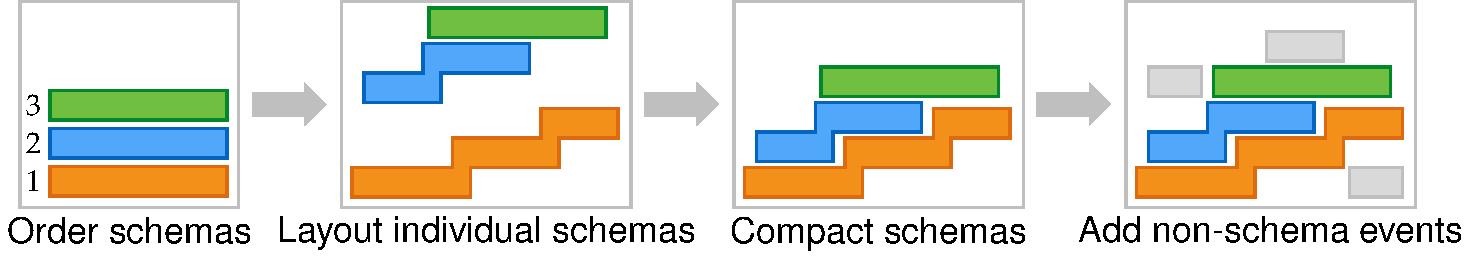
\includegraphics[width=\linewidth]{layout-overview}
\caption{The SchemaLine algorithm: First, the order of schemata is computed. Second, the layout of each schema is generated independently. Third, schemata are stacked together to save display space without changing order. Finally, events that do not belong to any schema are added.}
\label{fig:layout-overview}
\end{figure}

% \vspace{0.8cm}
\subsubsection{Schema Orders}
\label{sub:layout-order}
It is not always possible to have schemata that share events placed next to each other. For example, if three schemata all share events with each other, then in any order two of them will always be separated by the third schema. Our algorithm uses a strategy that prioritizes pairing of schemata according to how many events they share. To do this, we map the problem to graph path finding as below. Given a set of schemata $S$, we create an undirected graph $G = (V,E)$, where each vertex $v_i$ represents a schema $s_i \in S$. The weight of an edge $e_{ij}$ is the number of events shared by schemata $s_i$ and $s_j$. Finding a schema order with the maximum number of shared nodes placed next to each other becomes finding a path with maximum weight connecting all vertices in $G$. This classic longest path finding problem is NP-hard. The number of schemata we plan to support is at most eight due to the limitation of the small number of colors that human can distinguish. Therefore, we simply use brute-forte algorithm to find the path.

%We create another undirected graph $G' = (\emptyset,\emptyset)$ to store such a path. For each edge $e \in E$, in the decreasing order of its weight, if there is no path between the two end vertices of $e$ in $G'$ and the degrees of them are both less than two (otherwise it is not a path in $G'$), add $e$ to $G'$. The process stops when all vertices in $G'$ are connected or there are no remaining edges in $E$. As a result, we can either have one path connecting all vertices or multiple paths of sub-graphs in $G'$. These sub-graphs are disconnected; therefore, they can be joined in any order. An illustration of this algorithm is shown in Fig.~\ref{fig:layout-order-example}.
%
%\begin{figure}[H]
%\centering
%\includegraphics[width=\linewidth]{layout-order-example}
%\caption{Schema order algorithm. There are five schemata $A$, $B$, $C$, $D$, $E$, and four pairs of them have shared events as shown in $G$. Another graph $G'$ is initialized as an empty graph and edges from $G$ are added into $G'$ in decreasing order of weights: $AB$, $AC$, $CD$. Edge $AE$ cannot be added into $G'$ because the degree of $A$ is already equal to two. As the result, we have two possible paths: $B-A-C-D-E$ or $D-C-A-B-E$.}
%\label{fig:layout-order-example}
%\end{figure}

%\begin{algorithm}
%	\caption{Order Schemata}
%	\label{alg:orderSchemata}
%
%	\textbf{Input: } A set of schemata $S$.\\
%	\textbf{Output: } A ordered set $P$ with all the schemata in $S$.
%	
%	\begin{algorithmic}[1]
%		\State $G = (V,E)$;
%		\Statex \Comment{For each schema $s_i$, there is a vertex $v_i \in V$}
%		\Statex \Comment{For each pair of vertices $(v_i, v_j)$, there is an undirected edge $e_{ij} \in E$ }
%		\Statex \Comment{$w_{ij}$, the \emph{weight} of an edge $e_{ij}$, is the number of events the two schemata share}
%		\State $G' = (V,\emptyset)$ \Comment{store the schema order as a path}
%		\State Order $E$ by edge weight in descending order
%		\For {$i \leftarrow 0; i<|E|; i++$}		
%			\Statex \Comment{$v^0,v^1$: the two vertices of $e_i$}
%			\If {$w_i>0$}
%				\If {there is no path between $v^0$ and $v^1$ in $G'$ \textbf{and} the degree of $v^0$ and $v^1$ in $G'$ are both less than two}
%					\State Add $e_i$ to $G'$
%					\If {all vertices are connected in $G'$}
%						\State \textbf{return} the path $P$ in $G'$
%					\EndIf
%				\EndIf
%			\Else
%				\State \textbf{break} \Comment{early exit}
%			\EndIf
%		\EndFor
%		\State Connect all the sub-graphs in $G'$ with more than one vertex into a path;
%		\State $P \gets$ the current path in $G'$
%		\State Order remaining vertices that are not in $P$ by their schema length and append them to $P$;
%	\end{algorithmic}		
%\end{algorithm}

% \vspace{0.4cm}
\subsubsection{Individual Schema Layout}
\label{sub:layout-schema}
The second step of the algorithm produces the layout of each schema. Events shared by multiple schemata are replicated for each of them; therefore, the layout of each schema can be generated independently. Events within a schema are sorted chronologically so that they can be added from left to right. The algorithm works by adding one event at a time: the new event will stay at the same horizontal level as the previous one if it can, otherwise it will move up one level. When a event $n_i$ has the same time as the previous $n_{i-1}$, it needs to be moved up one level because they must have the same x-coordinate. Otherwise, if $n_i$ intersects with $n_{i-1}$, an attempt is made to shift $n_{i-1}$ to the left to make space for $n_i$ as discussed below. If the shifting is successful, the event stays in that level; otherwise, the event needs to move up one level.

%\vspace{-4mm}
\paragraph*{Shifting Events}
To address the issues of scalability and efficient use of space, accuracy of the event position can be sacrificed. For each event, its $x$-coordinate is initially set at event time ($C1$). Then, events can be shifted horizontally to the left by a limited amount, to make room for events that are after it temporally. An event can be rendered at the non-accurate position scaled with its time. However, to keep the event close to the accurate position, we set the maximum distance that a event can shift to its width. As a result, the event still overlaps with its time point on the timeline and provides reasonable indication to viewers of its true position. When shifting, it is crucial to maintain the relative order between the shifting event and other events ($C2$). For example, if event $n_i$ was to the left of $n$ before the shifting, it should remain on the left afterwards. Another important condition is that there is no intersection with any other event after the shifting ($C3$). An illustration of this algorithm is shown in Fig.~\ref{fig:layout-schema-example}.

%\begin{figure}[H]
%\centering
%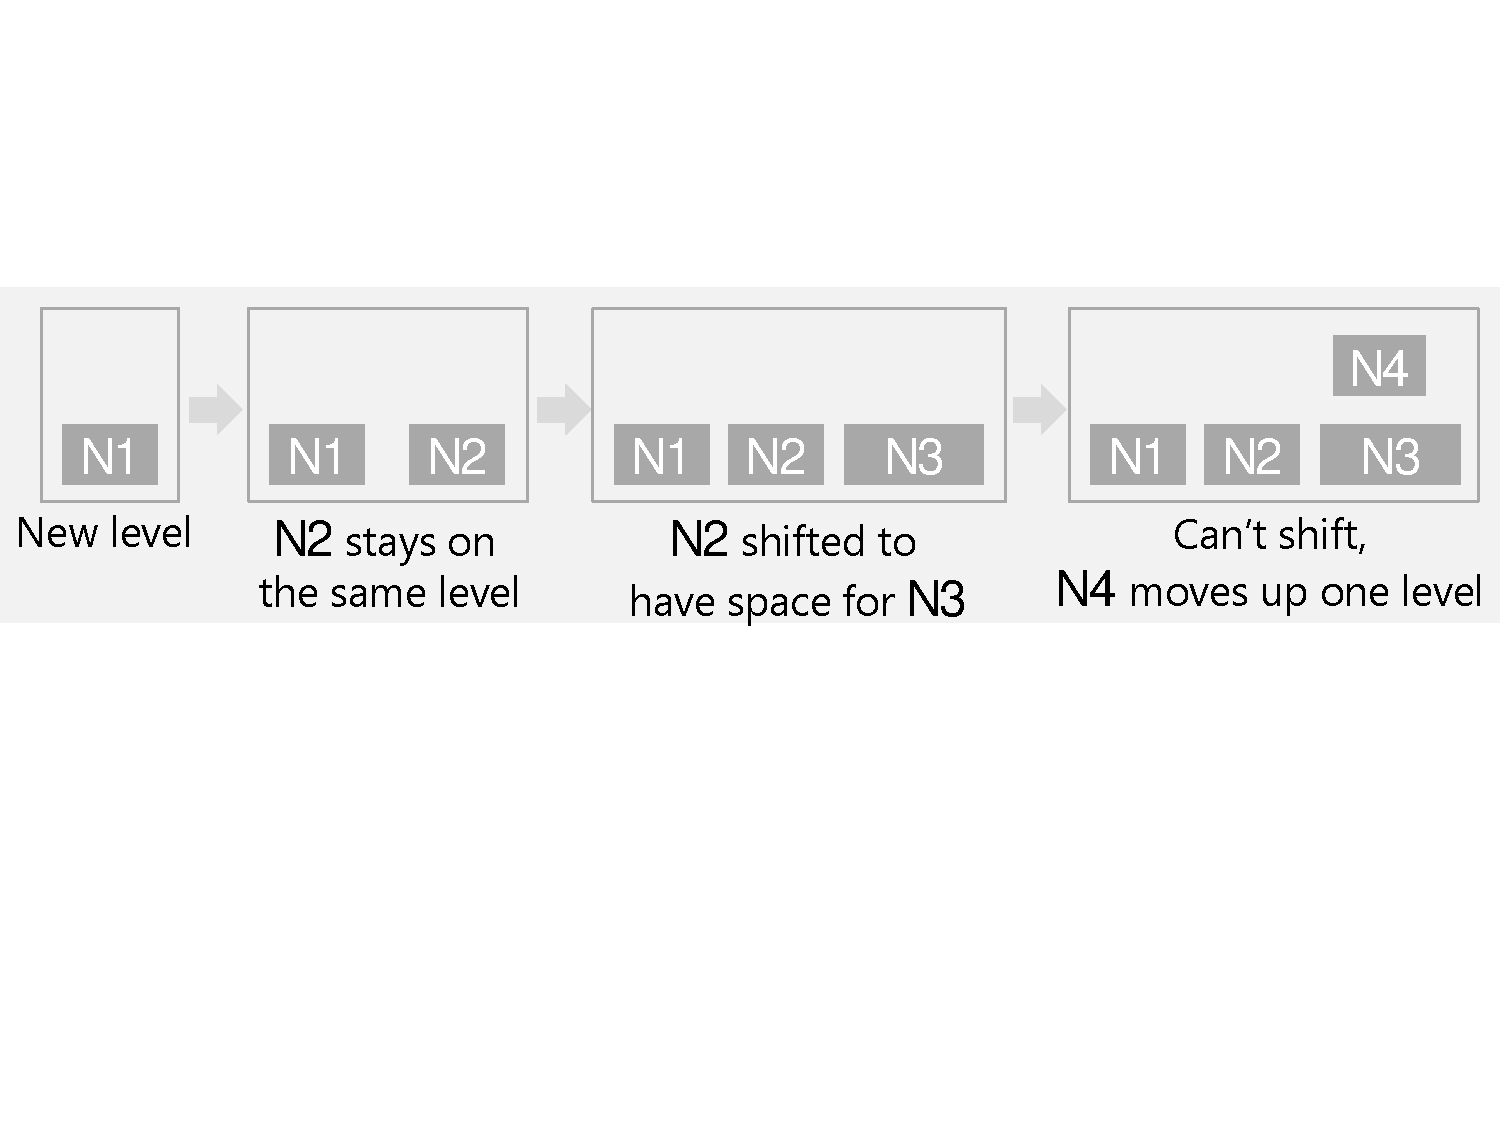
\includegraphics[width=\linewidth]{layout-narrative-example}
%\caption{Schema layout algorithm. Four events $N1$, $N2$, $N3$, $N4$ will be added to the schema stripe in chronological order. $N1$ is positioned at its accurate event time. $N2$ can stay in the same level as $N1$ because it does not intersect with $N1$. $N3$ intersects with $N2$ but the intersection width is small enough so that $N2$ can be shifted to the left to let $N3$ stay in the same level as well. However, $N4$ needs to move up one level because the width of its intersection with $N3$ is longer than that of $N1$ and $N2$, i.e., they cannot be shifted.}
%\label{fig:layout-schema-example}
%\end{figure}

%\begin{algorithm}
%	\caption{Schema Layout}
%	\label{alg:allocateSchemata}
%
%	\textbf{Input} 
%	\begin{itemize}
%		\item A set of schemata $S$. Each schema is a set of related events. A event $n_i$ has a time $t_i$, which is when the event that the event refers to happened. One event can belong to multiple schemata.
%	\end{itemize}
%	
%	\textbf{Output}
%	\begin{itemize}
%		\item A timeline $T$ that covers the timespan of all events. Its minimum and maximum time point are $T_{min}$ and $T_{max}$ respectively. Its width is $T_{width}$.
%		\item A set of event rectangles, one for each event in $S$. The rectangle for event $n_i$ has its  bottom-left corner at $(x_i, y_i)$, with a width $w_i$. All rectangles share the same height $h$.  
%		\item All the event rectangles should meet the conditions mentioned at the beginning of this section, and when a event $n_i$ is moved from it preferred horizontal position, its $x$-coordinate $x_i$ should meeting the following condition:
%		$$x_i \leq x_t \leq x_i+w_i$$ where $x_t = (t_i-T_{min})/(T_{max}-T_{min})*T_{width}$ is the preferred position.
%	\end{itemize}		 
%	
%	\begin{algorithmic}[1]
%		\State $T_{min} \leftarrow \min(t_i),~T_{max} \leftarrow \max(t_i),~\forall n_i \in N$
%		\For {$i \leftarrow 0; i<|N|; i++$} 
%			\State $x_i \gets (t_i-T_{min})/(T_{max}-T_{min})*T_{width}$
%		\EndFor
%		
%		\State Order schemata in $S$ using Algorithm \ref{alg:orderSchemata}
%		
%		\State $P \leftarrow \emptyset$
%		\Comment{the set of rectangles with allocated positions}	
%		\State $l \leftarrow 0$ \Comment{vertical level}
%%		\Statex \Comment{Intially shared events are duplicated for each schema}
%		\For {$i \leftarrow 0; i<|S|; i++$} 
%			\State Sort events in $s_i$ in the ascending order of their event time
%			\For {$j \leftarrow 0; j<|s_i|; j++$} 
%				\State Update $x_j$ to maintain its relative order
%				\State $y_j \leftarrow l$
%%				\Comment{explain in text how to map level $l$ to $y$-coordinate}
%				\If {$t_j = t_{j-1}$}
%					\State $y_j \leftarrow ++l$
%				\Else
%					\State $w \gets$ intersection width of $n_j$ and $n_{j-1}$
%					\If {$w > 0$} 
%						\If {\Call{shiftNote}{$n_{j-1}$, $P$, $w$} fails}
%							\State $y_j \leftarrow ++l$
%						\EndIf
%					\EndIf
%				\EndIf
%				\State $P \leftarrow P \cup \{n_j\}$
%			\EndFor
%			\State $l++$
%		\EndFor
%	\end{algorithmic}
%\end{algorithm}
%
%\subsubsection{Shift Events (Algorithm \ref{alg:shiftNote})}
%This function checks if a event $n$ can be shifted towards left by amount $d$. Besides making sure $n$ does not intersect with any event after the shifting, the algorithm also checks:
%\begin{itemize}
%	\item If any event share the same time as $n$ will intersect with anything after the shift.
%	\item If the relative order of any affected event is preserved.
%\end{itemize}
%The pseudo code is in Algorithm~\ref{alg:shiftNote}. Because the event is only shifted to the left, $P_L$ is the only set of events may be affected. Events having the same time (set $C$ in line 4) is checked. If there exists a event that needs to be shifted by more than its width, the function fails and all event positions keep unchanged (line 8). Next, the rest of $P_L$ is processed quite similarly, except that the shift distance is unknown yet. There are two constraints that need to be considered. The first distance is the intersection width between the current looping event and the event in the same level that has just shifted in the previous loop. The second distance is to maintain the relative order with the previous event, which is not on the same level. The total of distance to shift is the maximum of these two kinds of distance.

%\begin{algorithm}
%	\caption{Shift Note}
%	\label{alg:shiftNote}
%	
%	\textbf{Input} {
%		\begin{itemize}
%			\item $n$: the event needs to be shifted
%			\item $P$: a set of allocated events
%			\item $d$: the distance that $n$ needs to be shifted towards its left
%		\end{itemize}
%	}
%
%	\textbf{Output} {
%		\begin{itemize}
%			\item $FALSE$, if shifting $n$ fails.
%			\item $TRUE$, if shifting $n$ succeeds. Also update the position of $n$ and other shifted events in $P$.
%		\end{itemize}
%	}
%	\begin{algorithmic}[1]
%	\Function {shiftNote}{$n$, $P,d$}
%		\State $P_L \leftarrow $ the set of events to the left of $n$
%%		\Comment{Define in the text that a schema is to the left of a event if it intersects the event level to the left of the event.}
%		\State Sort events in $P_L$ by time in descending order (right to left)
%		\State $C \gets$ all events in $P_L$ with the same time as $n$
%		\If {all events in $C$ can be shifted by $d$}
%			\State Shift all events in $C$ by $d$
%		\Else \State \textbf{return} FALSE
%		\EndIf
%		\For {$i \gets 0;i < |P_L\setminus C|; i++$}
%			\State $C \gets $ the set of events having the same time with $n_i$
%			\State $d1 \gets $ $\max$(the intersection between event in $C$ and the event to its the right)
%			\State $d2 \gets max(x_i - x_{i-1},0)$ \Comment maintain relative order with $n_{i-1}$
%			\State $d=max(d1,d2)$
%			\If {all events in $C$ can be shifted by $d$}
%				\State Shift all events in $C$ by $d$
%			\Else 
%				\State Revert all the events in $P$ to their original position
%				\State \textbf{return} FALSE
%			\EndIf
%		\EndFor
%		\State \textbf{return} TRUE
%	\EndFunction
%	\end{algorithmic}
%\end{algorithm}

\subsubsection{Schemata Compact}
\label{sub:layout-compact}
In the third step, the algorithm stacks schemata in the order computed in the first step to produce a compact visualization. For example, if two schemata cover non-overlapping time ranges, they can be placed in the same level to save display space. 

The group of schemata that share events is added to the SchemaLine first. Their relative ordering top to bottom is fixed and each schema is pushed towards the bottom as much as possible to save display space. After this, schemata without any shared event are added, again from bottom up to find the lowest level possible.

%\begin{algorithm}
%	\event[p]{Not implemented yet}\caption{Compact Schemata}
%	\label{alg:CompactSchemata}
%
%	\textbf{Input: } A set of schemata $S$ to be vertically Compacted.\\
%	\textbf{Output: } A Compacted set of schemata
%	
%	\begin{algorithmic}[1]
%		\For{$i \leftarrow 1; i<|S|; i++$}
%			\If {$s_i$ is not sharing event with any other schemata}
%				\State $startLevel \gets 0$
%			\Else
%				\State $startLevel \gets $ the beginning level of events in $s_{i-1}$
%			\EndIf
%			\State $l_i \leftarrow$ the beginning level of events in $s_i$
%			\For {$l \gets startLevel;~l \le l_i; ~l++$}
%				\State Move $s_i$ to level $l$
%				\If {$s_i$ stays in the link between two share events}
%					\State \textbf{continue}
%				\Else
%					\If {$s_i$ intersects with any schemata $s_{i-1} \rightarrow s_0$}
%						\If {\Call{shiftNote}{} successfully}
%								\State Move $s_i$ to level $l$
%								\State \textbf{break}
%						\EndIf
%					\Else
%						\State Move $s_i$ to level $l$
%						\State \textbf{break}
%					\EndIf
%				\EndIf
%			\EndFor
%		\EndFor
%	\end{algorithmic}
%\end{algorithm}

\begin{figure}[ht]
\centering
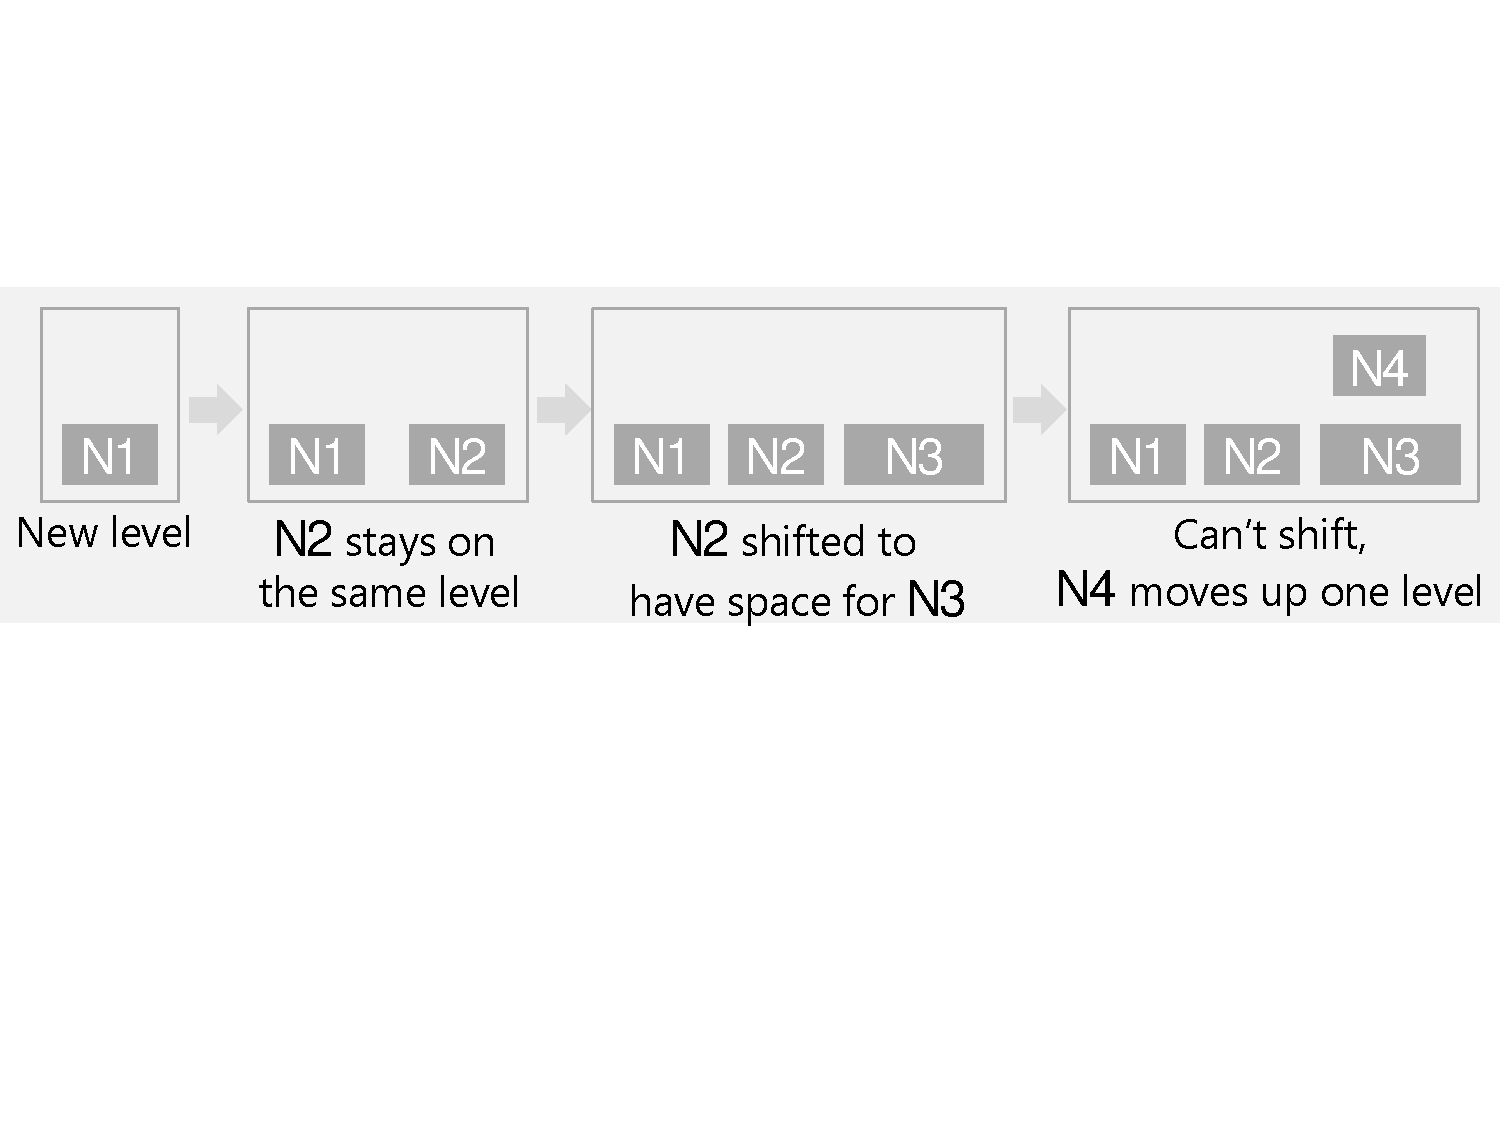
\includegraphics[width=\linewidth]{layout-narrative-example}
\caption{Schema layout algorithm. Four events $N1$, $N2$, $N3$, $N4$ will be added to the schema in chronological order. $N1$ is positioned at its accurate event time. $N2$ can stay in the same level as $N1$ because it does not intersect with $N1$. $N3$ intersects with $N2$ but the intersection width is small enough so that $N2$ can be shifted to the left to let $N3$ stay in the same level as well. However, $N4$ needs to move up one level because the width of its intersection with $N3$ is longer than that of $N1$ and $N2$, i.e., they cannot be shifted.}
\label{fig:layout-schema-example}
\end{figure}

\subsubsection{Non-schema Events}
\label{sub:layout-non-schema}
This last step allocates events that do not belong to any schemata. Events are sorted chronologically so that they are added to the SchemaLine from left to right. The ideal $x$-position is the event time, but an event can be shifted as described in Section~\ref{sub:layout-schema}. An event always begins at the lowest level and moves upward until there is enough space for it: that is, until it does not intersect with any other schema or events after possible horizontal shifting. 

%\begin{algorithm}
%	\caption{Add Non-Schema Events}
%	\label{alg:addNonSchemaEvents}
%	\textbf{Input} {
%		\begin{itemize}
%			\item $N$: a set of events not in any schema.
%			\item $S$: a set of schemata with allocated position.
%			\item $T$: a timeline covering all events in $N$ and $S$.		
%		\end{itemize}
%	}	
%	\textbf{Output}
%	Updated position of events in $N$ such that they meet the requirements listed in the \emph{output} of Algorithm~\ref{alg:allocateSchemata}.
%		
%	\begin{algorithmic}[1]
%		\State Sort events in $N$ by ascending time
%		\For {$i \leftarrow 0; i<|N|; i++$} 
%			\State $x_i \leftarrow (t_i-T_{min})/(T_{max}-T_{min})*T_{width}$
%			\State $l \leftarrow 0$
%			\While {true} 
%				\State $y_i \leftarrow l$
%				\If {$n_i$ intersects with event $n$ in $S$ }
%					\State $leftNode \gets $ the left event between $n_i$ and $n$
%					\State $w \gets $ the intersection width between $n_i$ and $n$
%					\If {\Call{shiftNote}{$leftNode$, $S$, $w$} successfully}
%						\State \textbf{break}
%					\EndIf 
%				\Else
%					\If {$n_i$ does not intersect with any schemata in $S$}
%						\State \textbf{break}
%					\EndIf
%				\EndIf
%				\State $l++$
%			\EndWhile
%		\EndFor
%	\end{algorithmic}
%\end{algorithm}

\subsection{SchemaLine Outline}
\label{sub:schema-outline}
In this section, we describe the algorithm to produce a polygonal outline covering all the event rectangles within a schema. We decided to use only horizontal or vertical line segments to keep the outline simple. The polygonal path $P_n$ of a schema that contains $n$ event rectangles $R_1, R_2, ..., R_n$, ordered from left to right, is determined as follows:
\[
P_n=
\begin{cases}
R_1, & n=1 \\
P_{n-1} \oplus R_n, & n > 1
\end{cases},
\]
where $\oplus$ is the \textit{merge operator} that merges a polygonal path and a rectangle into a new polygonal path. 

A polygonal path is simply represented as an array of vertex coordinates. As the above formula demonstrates, this array will be incrementally extended by adding each rectangle individually. As described in the schema layout algorithm (Section \ref{sub:layout-schema}), when adding a new event into an existing schema, the event either has the same level as the previous event of the schema or moves up one level. Polygonal path extension is simple; however, it needs to extensively cover all possible cases to produce a nice path. Fig.~\ref{fig:outline} shows five different cases that need to be considered when merging a polygonal path and a rectangle.

\begin{figure}[ht]
	\centering
	\subcaptionbox{Basic case 1 ($B1$): new rectangle $R3$ is on the right side of the path.}{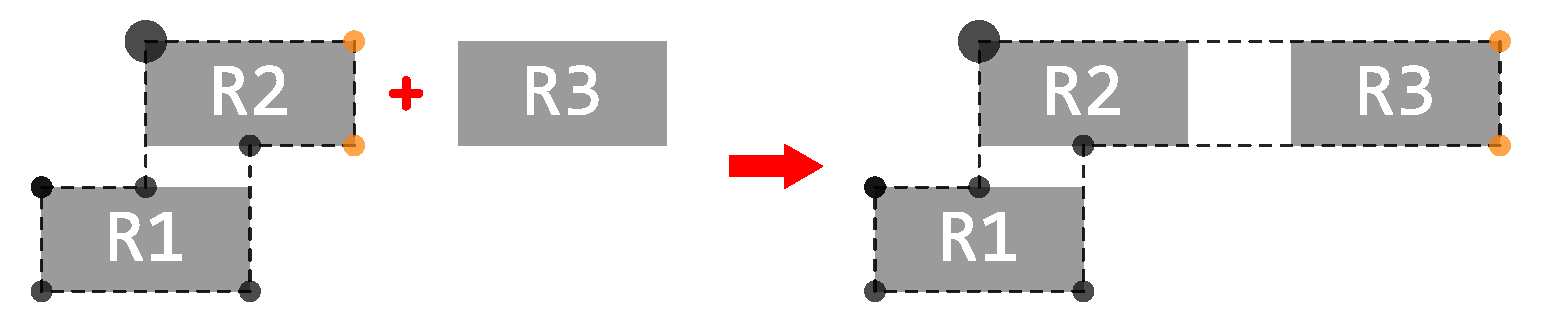
\includegraphics[width=0.6\columnwidth]{example-right}}
	\hfill
	\subcaptionbox{Basic case 2 ($B2$): new rectangle $R3$ is on top of the path.}{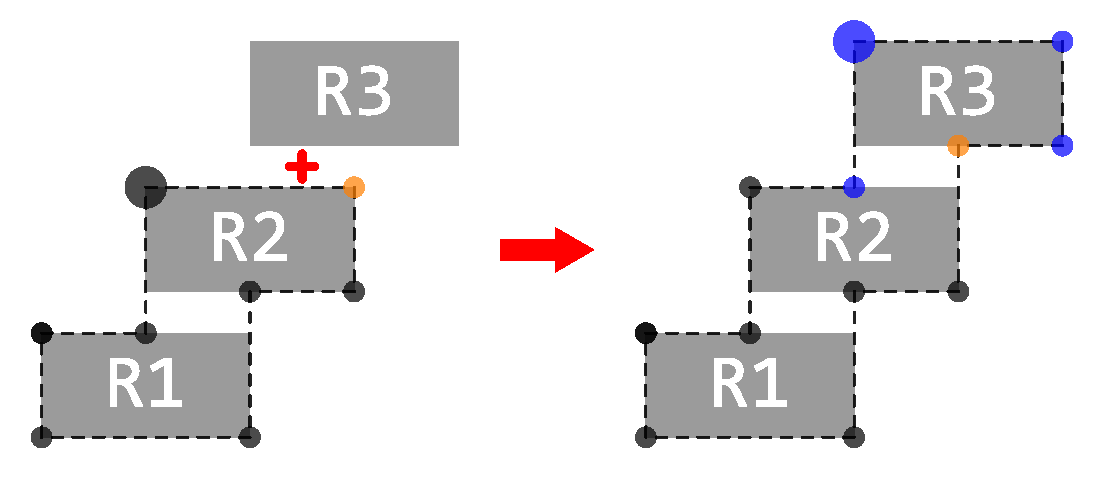
\includegraphics[width=0.36\columnwidth]{example-up}}
	\subcaptionbox{Special case of $B1$ when right-side of $R3$ is shorter than right-side of $R2$.}{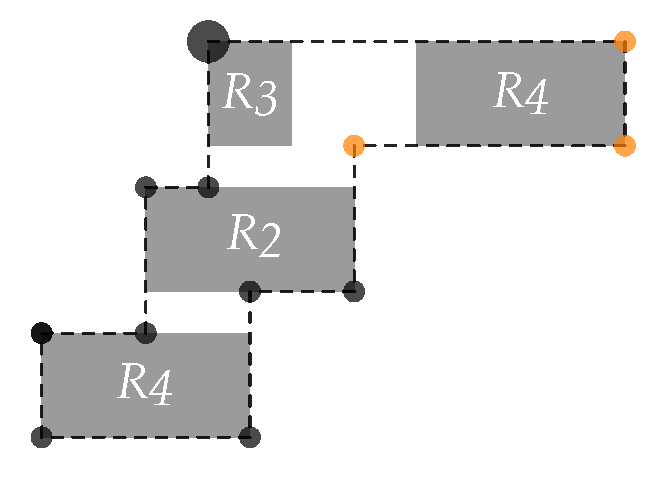
\includegraphics[width=0.42\columnwidth]{example-right-shorter}}
	\hfill
	\subcaptionbox{Special case of $B2$ when left-side of $R3$ is close to left-side of $R2$.}{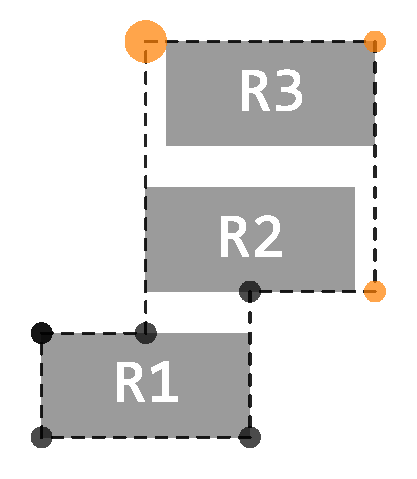
\includegraphics[width=0.26\columnwidth]{example-up-smoothing}}
	\hfill
	\subcaptionbox{Special case of $B2$ when right-side of $R3$ is shorter than right-side of $R2$.}{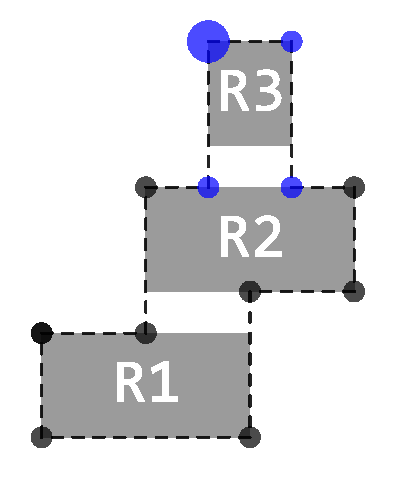
\includegraphics[width=0.25\columnwidth]{example-up-shorter}}
	\caption{Five possible cases when a new rectangle into the polygonal path. Big circle indicates the pivot vertex of the path (top-left corner of the last rectangle). Orange circles indicate updated vertices, and blue circles indicate newly added vertices of the polygonal path.}
	\label{fig:outline}
\end{figure}


%The polygonal path contains an array of vertices and an index of the top-left corner of the last rectangle in that array, the \textit{top-left-vertex}. As described in the schema layout algorithm (Section \ref{sub:layout-schema}), when adding a new event into an existing schema, the event either has the same level as the previous event of the schema or moves up one level. Therefore, the merge operator only needs to handle two cases:
%\begin{itemize} \setlength{\itemsep}{0pt}
%\item RIGHT-CASE (Fig.~\ref{fig:outline-right}): the top-left-vertex remains, the two next vertices in the array are updated with two right-side corners of the rectangle.
%\item UP-CASE (Fig.~\ref{fig:outline-up}): four new vertices are added, the top-left-vertex is assigned to the top-left corner of the rectangle, and the next vertex in the array is updated.
%\end{itemize}
%
%\begin{figure}[ht]
%\centering
%\subfigure[RIGHT-CASE: Two vertices after the top-left-vertex are updated with the right-side corners of $R3$]{\label{fig:outline-right}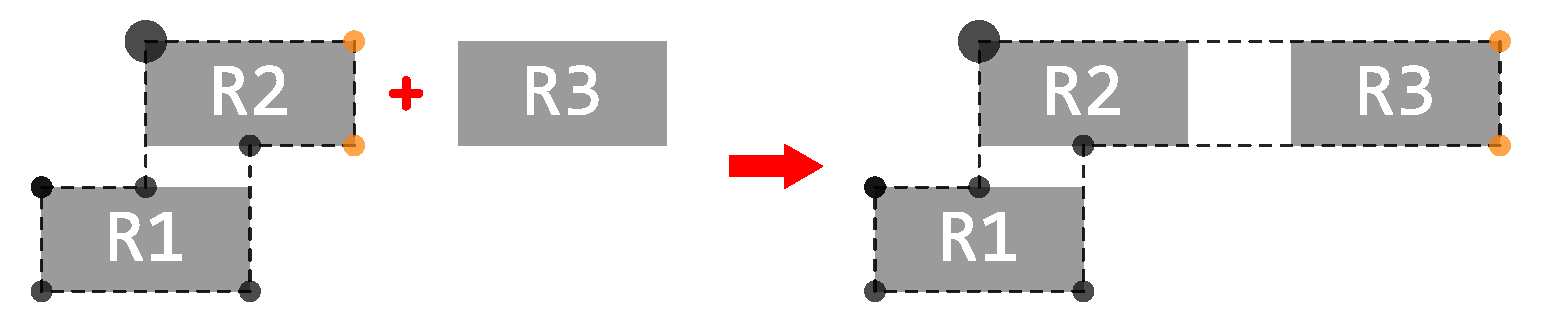
\includegraphics[width=.56\columnwidth]{example-right}} \hspace{0.2cm}
%\subfigure[UP-CASE: Four vertices from $R3$ are added, top-left-vertex is shifted two indices, and one verex is updated.] {\label{fig:outline-up}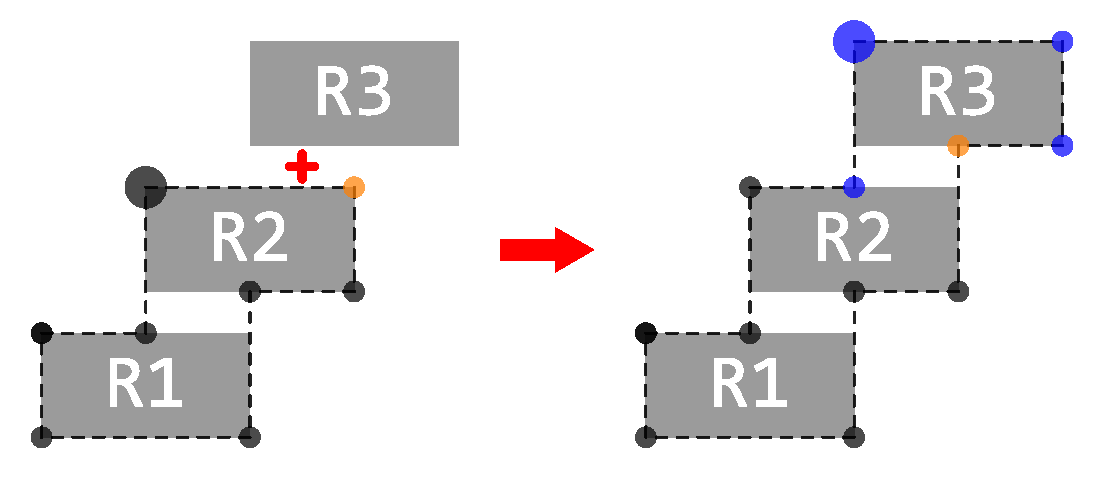
\includegraphics[width=.39\columnwidth]{example-up}}
%\caption{An illustration of two basic cases when merging a new rectangle $R3$ into the polygonal path. Big circle indicates top-left-vertex. Orange circles indicate updated vertices, and blue circles indicate newly added vertices of the polygonal path.}
%\label{fig:outline-basic-cases}
%\end{figure}
%
%Besides the two basic cases, there are three special cases. First, in the UP-CASE, when the left-side (or right-side) of the new event is close to the left-side (or right-side) of the previous event, these two events are merged together to produce a smooth path instead of creating a \textit{stair} between them (Fig.~\ref{fig:outline-up-smoothing}). Second, also in the UP-CASE, when the right-side of the new event is shorter than the right-side of the previous event, one of the four new vertices is different and there is no updated vertex compared to the standard UP-CASE (Fig.~\ref{fig:outline-up-shorter}). Third is the special RIGHT-CASE when it follows the special \textit{shorter} UP-CASE; there is one more vertex that needs to be updated compared to the standard RIGHT-CASE (Fig.~\ref{fig:outline-right-shorter}).
%
%\begin{figure}[ht]
%\centering
%\subfigure[Instead of creating a \textit{stair} from $R2$ to $R3$, vertices are updated to make the path smoother.  ]{\label{fig:outline-up-smoothing}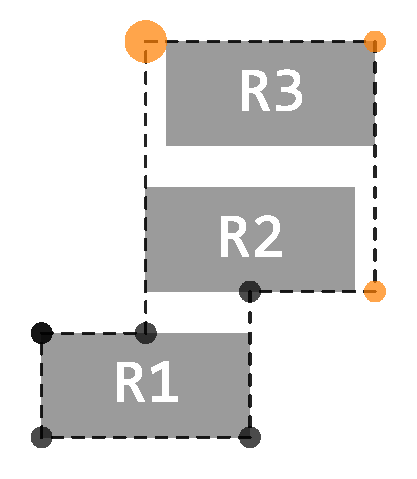
\includegraphics[width=.250\columnwidth]{example-up-smoothing}} \hspace{0.2cm}
%\subfigure[No updated vertex when the new event is shorter than the previous event.] {\label{fig:outline-up-shorter}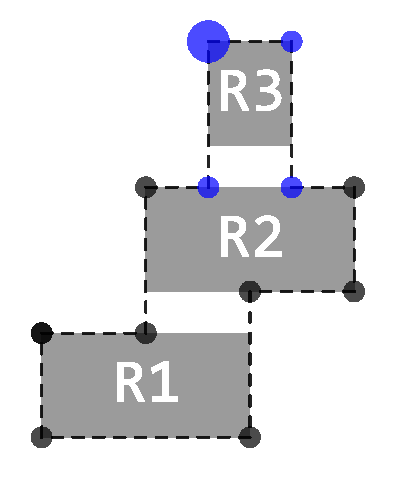
\includegraphics[width=.244\columnwidth]{example-up-shorter}}
%\hspace{0.2cm}
%\subfigure[One more vertex to update when the RIGHT-CASE follows the special \textit{shorter} UP-CASE.] {\label{fig:outline-right-shorter}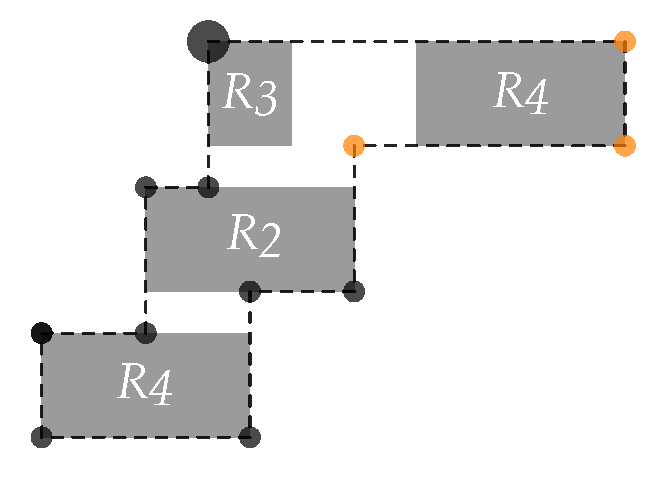
\includegraphics[width=.415\columnwidth]{example-right-shorter}}
%\caption{Three special cases when merging a new rectangle into the polygonal path. Note the difference in the update/new color-coded pattern compared to Fig.~\ref{fig:outline-basic-cases}.}
%\label{fig:outline-special-cases}
%\end{figure}

After producing a rectilinear path, the bends are made rounded to create a pleasing visualization (Fig.~\ref{fig:teaser}). The path is filled with the same stroke color but less transparency to make the border pop-out with a darker hue. The beginning of the path does not have the border to indicate that the path is open on that side and the reader should follow this direction. 



%According to Algorithm \ref{alg:allocateSchemata} of computing position for events in a schema, the schema polygon always stays in the same level or moves upward. Therefore, there are only four possible ways to connect the two adjacent events in the schema as shown in Fig.~\ref{fig:connectionTypes}. If two events are on the same level, they can be directly connected by horizontal segments (Fig.~\ref{fig:connectionType1}). If two events have the same x-coordinate and with, they can be directly connected by vertical segments (Fig.~\ref{fig:connectionType2}). If the right event is higher than the left event, the connection can be either right first and then up (Fig.~\ref{fig:connectionType3}), or up first and then right (Fig.~\ref{fig:connectionType4}). The connection type of event $n_1$ and $n_2$ is deeventd as $C(n_1,n_2)$
%
%The first stage of the algorithm is to find the connection types between all two adjacent events to minimize the number of bends of the polygon. In Fig.~\ref{fig:connectionTypes}, DIRECT-RIGHT and DIRECT-UP have zero bend; while RIGHT-UP and UP-RIGHT have one bend. The two former connection types are fixed; whereas, the two later types are flexible because we can choose either of them to advance from event to another. The connection type is composed of two parts; for example with RIGHT-UP, the first part is RIGHT and the second part is UP. Both the first part and the second part of DIRECT-RIGHT are RIGHT. Considering an example to connect three events $n_1$, $n_2$, $n3$ together, to minimize the number of bends, the first part of $C(n_2,n3)$ needs to match with the second part of the $C(n_1,n_2)$ to create a straight segment. For instance, if $C(n_1-n_2)$ is RIGHT-UP, then $C(n_2-n3)$ should be DIRECT-UP or UP-RIGHT. If $C(n_2-n3)$ is DIRECT-RIGHT, we need to accept one bend. The first step is traversing through the path and assigning fixed connection types (DIRECT-RIGHT, DIRECT-UP). Then, empty connection types are determined in a ``rear-front matching'' mechanism mentioned above to minimize the number of bends.
%
%\begin{figure}[ht]
%\centering
%\subfigure[DIRECT-RIGHT connection between two events in the same level] {\label{fig:connectionType1}\includegraphics[height=.28\columnwidth]{connection-type-1}} \hspace{0.05cm}
%\subfigure[DIRECT-UP connection if two events have the same x-coordinate and width] {\label{fig:connectionType2}\includegraphics[height=.28\columnwidth]{connection-type-2}} \hspace{0.05cm}
%\subfigure[RIGHT-UP connection: go right first and then bend up] {\label{fig:connectionType3}\includegraphics[height=.28\columnwidth]{connection-type-3}} \hspace{0.05cm}
%\subfigure[UP-RIGHT connection: go up first and then bend right] {\label{fig:connectionType4}\includegraphics[height=.28\columnwidth]{connection-type-4}}
%\caption{4 possible connection types between two events.}
%\label{fig:connectionTypes}
%\end{figure}
%
%The second stage of the algorithm is to generate a list of points constructing the polygon. This is done by traversing on the ``left'' side of the polygon and then going back, still on the ``left'' side. During the traversal, points at bends are added to the list. More specifically, the list consists of one starting point, bending points in the forward pass, two points needed when turning-back, bending points in the backward pass, and the ending point. Fig.~\ref{fig:outline-demo} shows an example of how the polygon is constructed with all four different connection types.
%
%\begin{figure}
%\centering
%\includegraphics[width=\linewidth]{outline-demo}
%\caption{An example of schema outline with all four different connection types. The connection type list is DIRECT-RIGHT---RIGHT-UP---UP-RIGHT---RIGHT-DIRECT-UP and produces three bends. The polygon consists of one starting point, three forward bending points, two turn-back points, three backward bending points, and one ending point. }
%\label{fig:outline-demo}
%\end{figure}


%\begin{algorithm}
%	\caption{Generate Schema Outline}
%	\label{alg:generateSchemaOutline}
%	\textbf{Input:} A schema $s$ containing a list of event rectangles.\\
%	\textbf{Output:} A orthogonal polygon covering all event rectangles in $s$ with least bends.
%	
%	\begin{algorithmic}[1]
%%		\Statex \Comment{Explain in the text a schema polygon is created by connecting its event rectangles.}
%		\State Order events in $s$ from left to right
%		\State $index \leftarrow $ the index of the first fixed connection between two events in the schema, either DIRECT-UP or DIRECT-RIGHT
%		\For {$i \leftarrow index; i > 0; i--$} 
%			\State Select the connection type between two events $n_i n_{i-1}$ to reduce bends
%		\EndFor
%		\For {$i \leftarrow index+1; i<|s|-1; i++$} 
%			\State Select the connection type between two events $n_i n_{i+1}$ to reduce bends
%		\EndFor
%		\State \textbf{return} the outline of $s$
%	\end{algorithmic}
%\end{algorithm}
